%\chapter{Problem and Its Background}
\chapter{INTRODUCTION}

\section{Background of the Study}

% AI Game engine prog p 415
Genetic algorithms are one of the many types of artificial intelligence
techniques that exist today. If implemented well, genetic algorithms can
evolve a computer controlled agent to perform adequately according to some
set criteria defined in a fitness function. However, a significant amount of 
time is required for the algorithm to evolve a population of individual solutions 
into an acceptable solution\cite{Schwab04}. The time it takes can range from
a few hours to a number of weeks, depending on the complexity of the game where
the agent must perform. This limitation makes them difficult or impractical to
use in the process of game development\cite{Schwab04}.

% refer to the bottom part of p 415 and top part of p 417 in AI game engine prog
The primary reasons genetic algorithms take up a lot of time are the number of 
possible solutions that must be tested given a specific generation, the time it 
takes to evaluate each of these possible solutions, and the number of generations 
that may be needed before arriving at a single or a number of acceptable solutions\cite{Schwab04}. 
One way to tackle the issue is by using faster processors in order to reduce the
overall computation time of the Genetic Algorithm. A better solution though would
be to process all the individuals in a single generation in parallel through the
use of threads. A computer processor is capable of a variety of things, but it can only process
one instruction at a time. This is where Graphics Processing Units, or GPUs, come in.
GPUs have been designed to execute a single set of instructions over numerous elements
of data, a technique known as ``Single-Instruction, Multiple-Thread\cite{pdf:NVCudaPrgGuide}.''
Not only do they have multiple processing units, each processing unit is also
capable of running several identical instructions simultaneously, making GPUs ideal
for highly parallel algorithms\cite{pdf:NVCudaPrgGuide}. It is our goal therefore to
show that GPUs can be used to evolve an optimized solution for the behavior of computer
controlled agents in a computer game at a rate that is much faster than those that are optimized
through the use of a CPU.

\begin{figure}
	\centering
		\graphicspath{{images/}}
		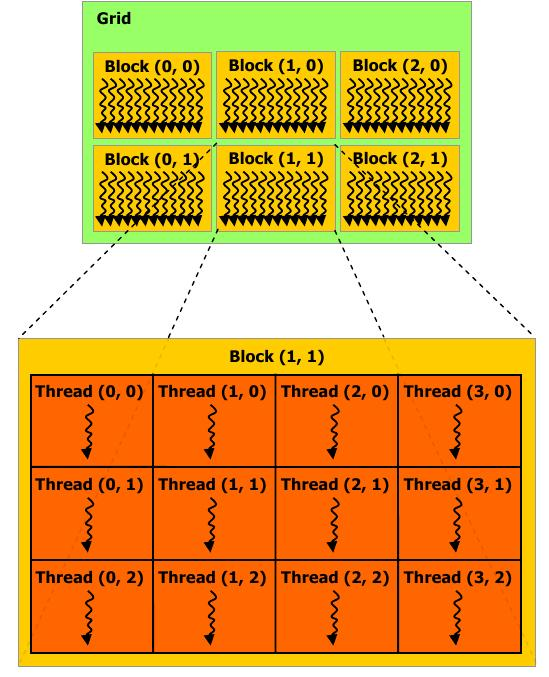
\includegraphics[width=450 pt]{gpu.jpg}
	\caption{Threads and thread blocks in a GPU}
	\cite{pdf:NVCudaPrgGuide}
	\label{fig:gpu_diagram}
\end{figure}

\section{Research Objectives}

The objective of this study is to show that the GPU can be used to reduce the time
it takes to optimize game AI and thus make them more practical for use during the
development process of computer games. This research aims to do the following:

\begin{itemize}
 \item Illustrate the performance gains of using a GPU to optimize the AI with the
use of Genetic Algorithms.
\end{itemize}


\section{Research Question}

These are the questions that should be addressed in designing the application:

\begin{itemize}
 \item How should the AI be represented as a genome for the purpose of evolution in a genetic algorithm?

 \item How do we structure the game such that most of the code may be shared between
the actual game and the offline tool that utilizes the GPU?

 \item Under what specific criteria should we judge an individual solution for use in the
fitness function?

 \item How practical is this solution compared to a pure CPU implementation?
\end{itemize}


The following questions are for determining if the application proves our theory
in making use of GPUs for evolving AI solutions to a game:

\begin{itemize}
 \item How much faster is the GPU assisted solution as compared to the pure CPU
 version?
 
 \item How well did the evolved AI solutions perform in the actual game?
 
 \item Is it possible to re-use portions of the code for evolving the AI for other
 types of games?
\end{itemize}

\section{Scope and Limitations}

DUR

\section{Significance}

Genetic algorithms have applications over a wide variety of fields.
Inspired by evolutionary biology, it can find the optimal solution
for a given problem.  For example, artificial neural networks , ANNs, are used in the manufacturing
industry to identify the best parameters for constructing a model.  Genetic 
algorithm based ANNs are found to be the best due to its time-saving potential\cite{Venkatesan08}.  
Another application can be found in the field of traffic control.  They used genetic algorithm to design an
optimal toll ring scheme\cite{Sumalee08}.
Other applications can be found in the field of AI.  For example, we can 
make more sophisticated AI using genetic algorithms.  These AIs will be smarter in the 
sense that it can ``learn''.  This can be very invaluable in a game due to making the AI a lot more challenging.  
With the age of graphics reaching its peak, the need for better AI starts being an
ingredient for a succesful commercial game\cite{Yue06}.  Because of the inherent ability
of genetic algorithms in learning, AIs can be made more robust.  They could 
display behaviors that were not seen in the previous playthrough.  Thus, 
this could make more challenging AIs after each playthrough.  This was made an 
example of through Megaman 2 in the boss fight against Air Man.  It kept trying different 
set of inputs to defeat Air Man.  Each generation performed better than the last 
until it reached Generation 13 whereby its fitness score didn't increase anymore\cite{website:Kuliniewicz09}.  


Other applications of genetic algorithm can be found in companies like First Quadrant Corp.
It is an investment management firm that used genetic algorithms to model yield on 
investment funds\cite{website:Davis}.  Through this method, they are have a ``significant improvement''
of over USD 128 Billion under investment\cite{website:Davis}.  Furthermore, in the field of Telecommunications, 
Cox Associates is using genetic algorithms for their cellular clients\cite{website:Davis}.  
As a result, they are saving millions of dollars.  Another application can be found 
in the field of traffic control, specifically in traffic lights and pedestrian crossing
control\cite{Turky09}.  

Various studies have already been done in the fields of genetic algorithm with some of the applications
being used commercially.
However, it would seem that there has yet to be any study done in improving genetic algorithms
using the GPU for Game AIs.  It has been proven that genetic algorithms are limited without
the processing power of the GPU\cite{Banzhaf09}.  Therefore, the processing power of the GPU can give better 
results because of its parallel structure.  Thus, it is possible to have a large population size.
With this, the AI can evolve and find better results , i.e., fitness scores, creating behaviors that are normally
unseen in normal situation.  It is here that we belive that we 
could make a contribution to the field of both Genetic Programming and Game Development (AI development).